\chapter{KESEHATAN LINGKUNGAN}
Faktor lingkungan mempunyai faktor yang sangat penting dalam proses timbulnya gangguan kesehatan baik secara umum maupun individual. Upaya pembinaan kesehatan lingkungan dan sanitasi dasar secara prinsip dimaksudkan untuk memperkecil atau meniadakan faktor terjadinya penyakit atau gangguan kesehatan akibat lingkungan yang kurang sehat. 

Bentuk upaya yang dilakukan dalam peningkatan kualitas lingkungan antara lain adalah melakukan pembinaan kesehatan lingkungan pada masyarakat dan institusi, survailen vektor, dan pengawasan tempat-tempat umum. Upaya kesehatan lingkungan diarahkan pada masyarakat dan institusi yang berpotensi mengancam kesehatan masyarakat yang dilakukan secara berkala. Kegiatan pembinaan yang dimaksud mencakup upaya pemantauan,penyuluhan dan pemberian rekomendasi terhadap aspek penyediaan fasilitas sanitasi dasar (air bersih dan jamban), inspeksi kesehatan bangunan mencakup pengolahan sampah, sirkulasi udara, pencahayaan, dan lain sebagainya.

Lingkungan sehat mencakup lingkungan permukiman, tempat kerja, tempat rekreasi, serta tempat dan fasilitas umum, harus bebas dari unsur-unsur yang menimbulkan gangguan, di antaranya limbah (cair, padat, dan gas), sampah yang tidak diproses sesuai dengan persyaratan, vektor penyakit, zat kimia berbahaya, kebisingan yang melebihi ambang batas, radiasi, air yang tercemar, udara yang tercemar, dan makanan yang terkontaminasi.

\section{PENGAWASAN SARANA AIR MINUM}
Setiap pelaksana penyelenggara air minum wajib menjamin air minum yang diproduksinya aman bagi kesehatan. Oleh karena itu pengawasan kualitas air minum, baik oleh internal maupun eksternal diperlukan agar masyarakat mendapatkan air minum yang tidak hanya layak, namun juga aman untuk dikonsumsi.

Pengawasan kualitas air minum aman adalah paya yang dilakukan untuk mengawasi kualitas air minum dari pelaksana penyelenggara air minum baik secara internal maupun eksternal terhadap air yang dihasilkan dan harus memenuhi syarat secara fisik, kimia, maupun mikrobiologi.
Penyelenggara air minum yang diawasi  meliputi:
\begin{itemize}
  \item BUMN/BUMD (misal PDAM) yang bergerak dalam bidang air minum perpipaan;
  \item UPT/UPTD yang bergerak dalam bidang air minum perpipaan;
  \item DAM, Pengelola Permukiman, Pengelola Rumah Susun;
  \item Kelompok Pengelola Sarana Air Minum (KPSAM) pedesaan/PAMSIMAS;
  \item BUMDes yang bergerak dalam bidang air minum perpipaan;
  \item Pengelola Kawasan Khusus; dan
  \item Pengelola Air Minum Untuk Kebutuhan Sendiri (BUKS).
\end{itemize}
Sarana air minum dikatakan memenuhi syarat mikrobiologi, fisik dan kimia jika :
\begin{itemize}
  \item Sarana air minum  yang masuk dalam kategori tinggi dan amat tinggi  berdasarkan hasil inspeksi kesehatan lingkungan telah dilakukan tindakan perbaikan; dan
  \item Sarana air minum yang masuk dalam kategori rendah dan sedang berdasarkan hasil inspeksi   kesehatan lingkungan telah diambil dan diperiksakan (diujikan) sampel airnya berdasarkan parameter fisik, kimia, mikrobiologi yang mana hasil pemeriksaannya (pengujiannya) memenuhi standar persyaratan kualitas air minum berdasarkan Permenkes No. 492 Tahun 2010 tentang  persyaratan kualitas air minum.
\end{itemize}

Pada tahun \tP terdapat 46,88\% sarana air minum yang diawasi/ diperiksa kualitas air minumnya sesuai standar (aman) (\autoref{fig:Cakupan-Air-Minum-Aman}).

\begin{figure}[H]
    \centering
    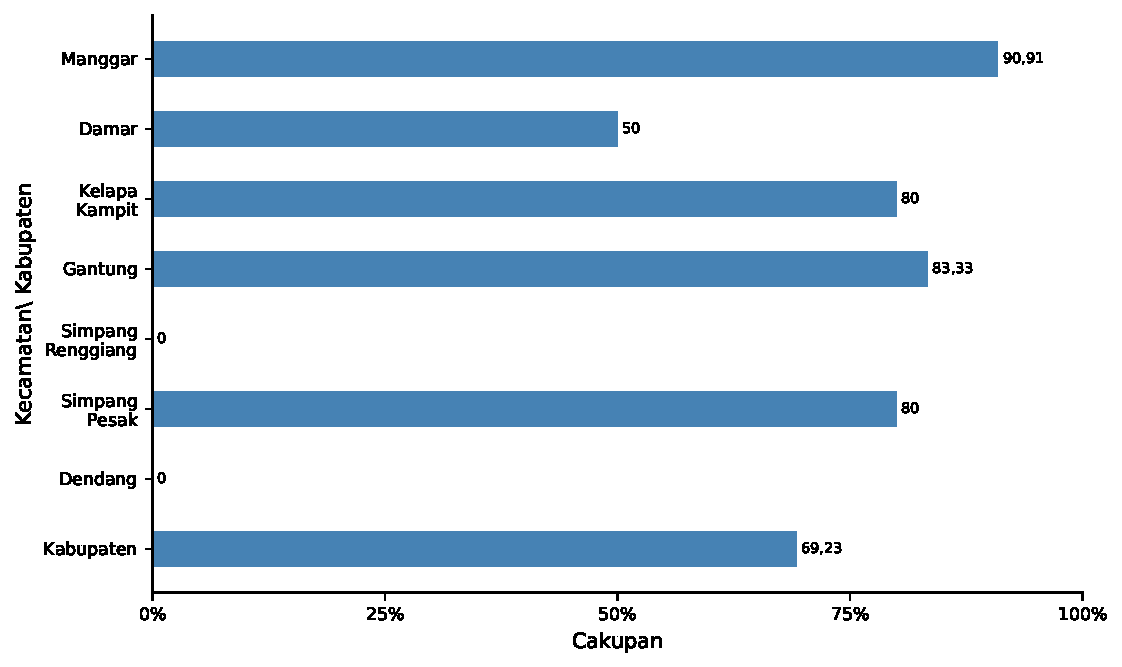
\includegraphics[width=0.85\textwidth]{bab_07/bab_07_01_airMinumAman}
    \caption{Cakupan Sarana Air Minum Aman di Kab. Belitung Timur Tahun \tP per Kecamatan}
    \label{fig:Cakupan-Air-Minum-Aman}
\end{figure}

\section{AKSES SANITASI}
Sanitasi yang baik merupakan elemen penting yang menunjang kesehatan manusia.
Sanitasi berhubungan dengan kesehatan lingkungan yang mempengaruhi derajat kesehatan masyarakat. 
Buruknya kondisi sanitasi akan berdampak negatif di banyak aspek kehidupan, mulai dari turunnya kualitas lingkungan hidup masyarakat, tercemarnya sumber air minum bagi masyarakat, meningkatnya jumlah kejadian diare dan munculnya beberapa penyakit. 

Sebuah rumah tangga dianggap telah memiliki akses sanitasi layak apabila fasilitas sanitasi yang digunakan memenuhi syarat kesehatan antara lain dilengkapi dengan leher angsa, tanki septik (\emph{septic tank})/ Sistem Pengolahan Air Limbah (SPAL), yang digunakan sendiri atau bersama.
Sebuah rumah tangga dianggap telah memiliki akses sanitasi aman apabila menggunakan fasilitas sanitasi rumah tangga milik sendiri menggunakan leher angsa dengan tangki septik yang
disedot setidaknya sekali dalam 3-5 tahun terakhir atau terhubung ke Sistem Pengolahan Air Limbah (SPAL) (kriteria 1).

Pada tahun \tP jumlah KK Kabupaten Belitung Timur yang memiliki akses pada
sanitasi layak adalah sebanyak 40.359 KK atau 97,06\%, sedangkan akses sanitasi aman adalah sebesar 1.435 KK atau 3,45\% (\autoref{fig:Cakupan-Akses-Sanitasi}), meningkat dari cakupan tahun 2019 sebesar 95,95\%.

\begin{figure}[H]
    \centering
    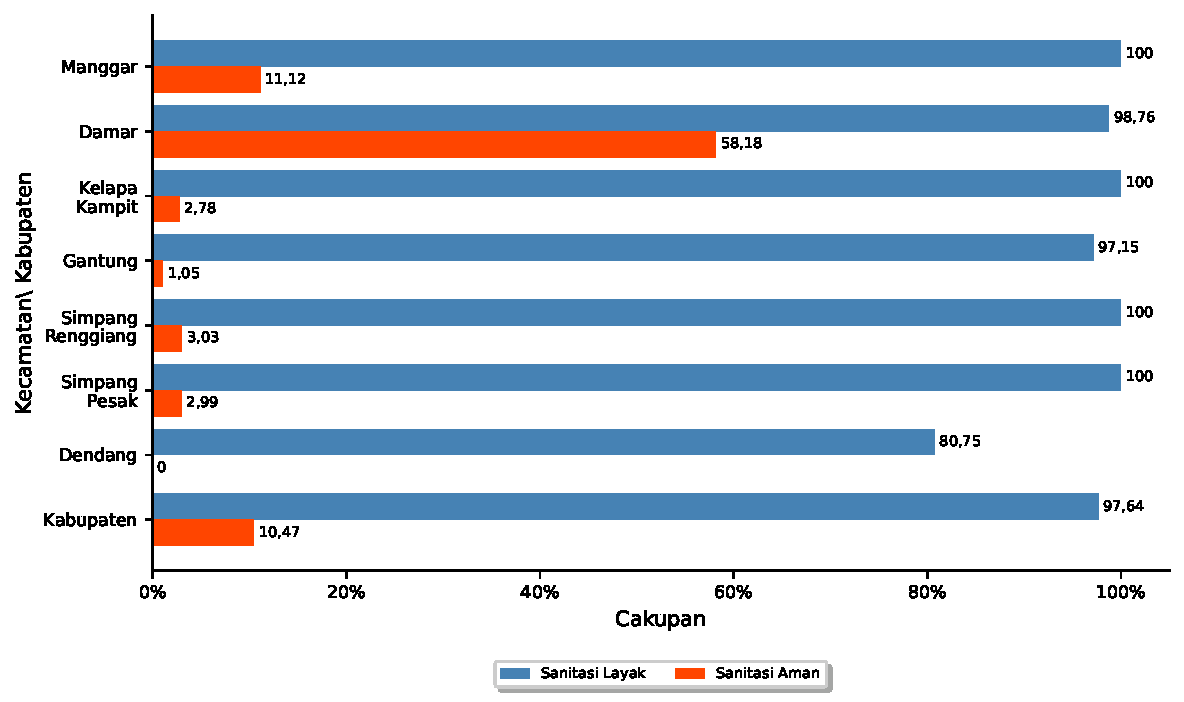
\includegraphics[width=0.85\textwidth]{bab_07/bab_07_02_aksesSanitasi}
    \caption{Cakupan Akses Sanitasi Layak di Kab. Belitung Timur Tahun \tP per Kecamatan}
    \label{fig:Cakupan-Akses-Sanitasi}
\end{figure}

\section{SANITASI TOTAL BERBASIS MASYARAKAT}
Sanitasi Total Berbasis Masyarakat (STBM) adalah pendekatan untuk mengubah perilaku higienis dan saniter melalui pemberdayaan masyarakat dengan cara pemicuan. 
Perilaku yang digunakan sebagai acuan dalam penyelenggaranaan STBM meliputi 5 pilar yaitu:
\begin{itemize}
	\item Stop Buang Air Besar Sembarangan (SBS);
	\item Cuci Tangan Pakai Sabun (CTPS);
	\item Pengelolaan Air Minum dan Makanan Rumah Tangga (PAMMRT);
	\item Pengelolaan Sampah Rumah Tangga (PSRT); dan
	\item Pengamanan Limbah Cair Rumah Tangga (PLCRT)
\end{itemize} 

Sebanyak 39 desa atau 100\% jumlah desa di Kabupaten Belitung Timur pada tahun \tP telah mencapai status Desa Stop BABS (SBS)/ \emph{Open Defecation Free} (ODF), yaitu desa yang penduduknya telah 100\% mengakses jamban sehat (\autoref{fig:Cakupan-Desa-SBS}).

\begin{figure}[H]
    \centering
    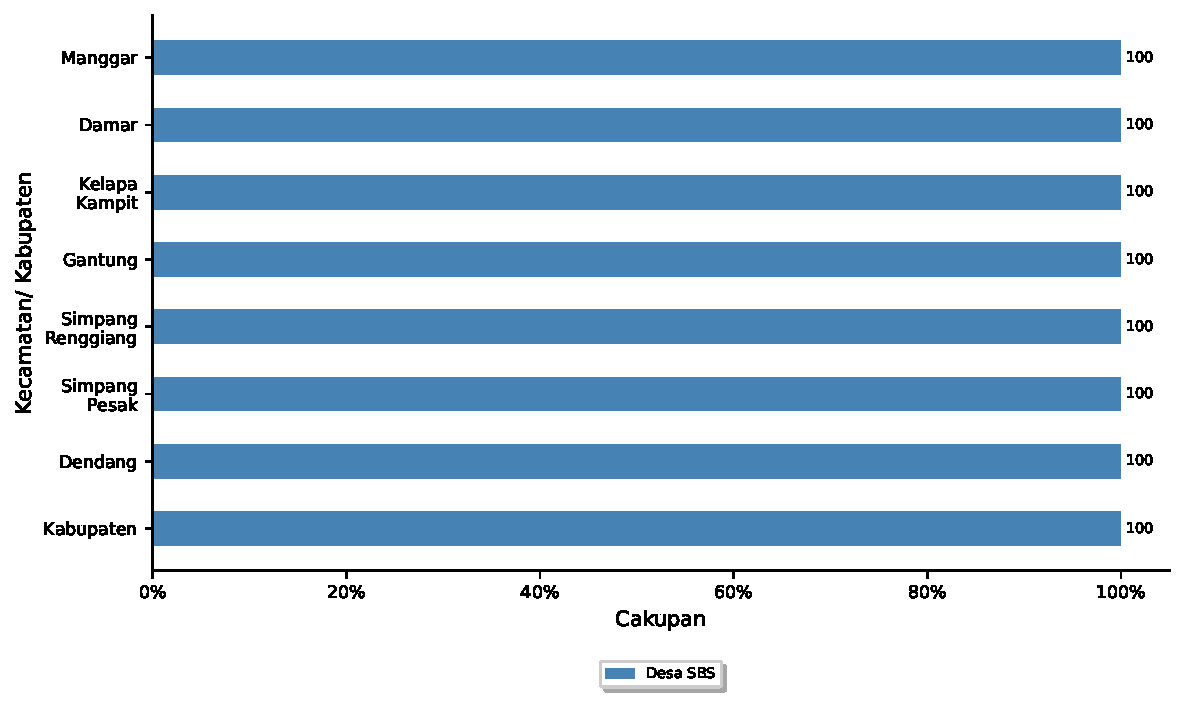
\includegraphics[width=0.85\textwidth]{bab_07/bab_07_03a_desaSBS}
    \caption{Cakupan Desa Stop BABS (ODF) di Kab. Belitung Timur Tahun \tP per Kecamatan}
    \label{fig:Cakupan-Desa-SBS}
\end{figure}

Sebanyak 1.198 KK atau 2,88\% KK di Kabupaten Belitung Timur pada tahun \tP telah memiliki akses rumah sehat, yaitu KK yang telah melakukan 5 pilar STBM (\autoref{fig:Cakupan-KK-Rumah-Sehat}).

\begin{figure}[H]
	\centering
	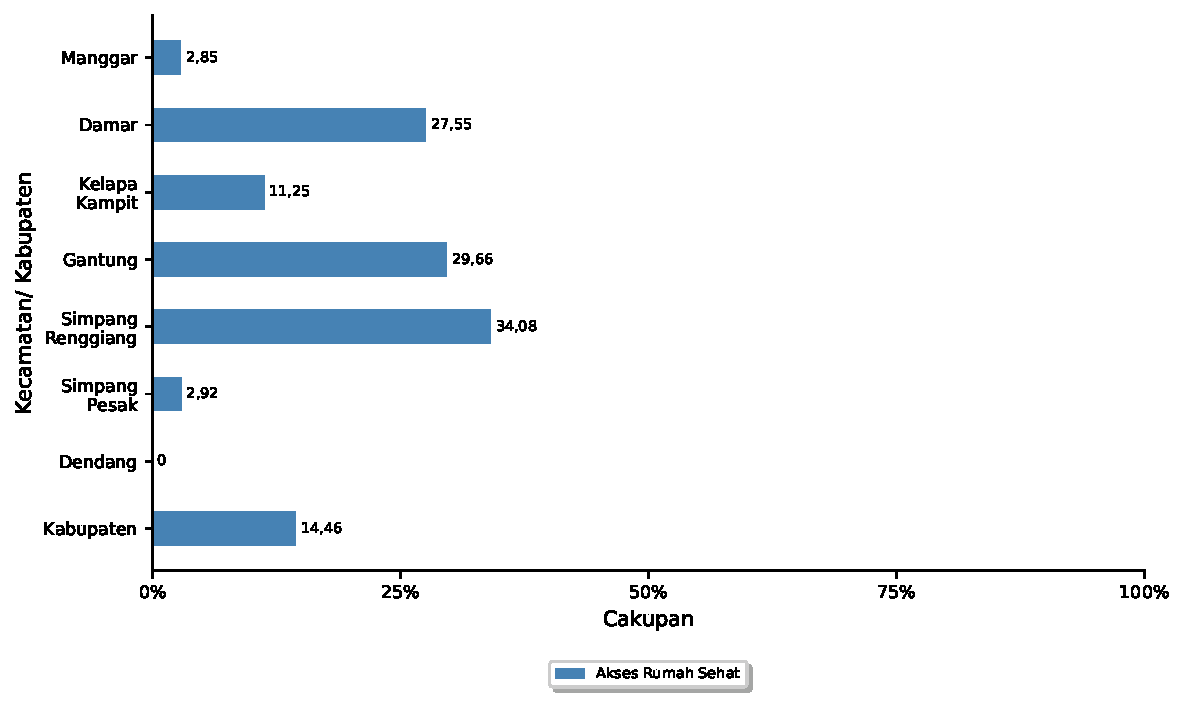
\includegraphics[width=0.85\textwidth]{bab_07/bab_07_03b_aksesRumahSehat}
	\caption{Cakupan KK Dengan Akses Rumah Sehat di Kab. Belitung Timur Tahun \tP per Kecamatan}
	\label{fig:Cakupan-KK-Rumah-Sehat}
\end{figure}

\section{PENGAWASAN TEMPAT DAN FASILITAS UMUM}
Tempat dan Fasilitas Umum (TFU) adalah lokasi, sarana, dan prasarana yang meliputi fasilitas kesehatan, fasilitas pendidikan, tempat ibadah, hotel, rumah makan dan usaha lain yang sejenis, sarana olahraga, sarana transportasi darat, laut, udara, dan kereta api, stasiun dan terminal, pasar dan pusat perbelanjaan, pelabuhan, bandar udara, dan pos lintas batas darat negara, dan tempat dan fasilitas umum lainnya. Pada profil kesehatan ini, TFU yang dilakukan pengawasan adalah sekolah, puskesmas dan pasar.

Pengawasan terhadap TFU dilakukan untuk meminimalisir faktor resiko sumber penularan bagi penyakit masyarakat yang memanfaatkan tempat-tempat umum.
Bentuk kegiatan yang dilakukan antara lain meliputi pengawasan kualitas lingkungan tempat-tempat umum secara berkala, bimbingan penyuluhan, dan saran perbaikan dalam peningkatan kualitas lingkungan yang sehat, serta pemberian rekomendasi TFU.

\begin{figure}[H]
    \centering
    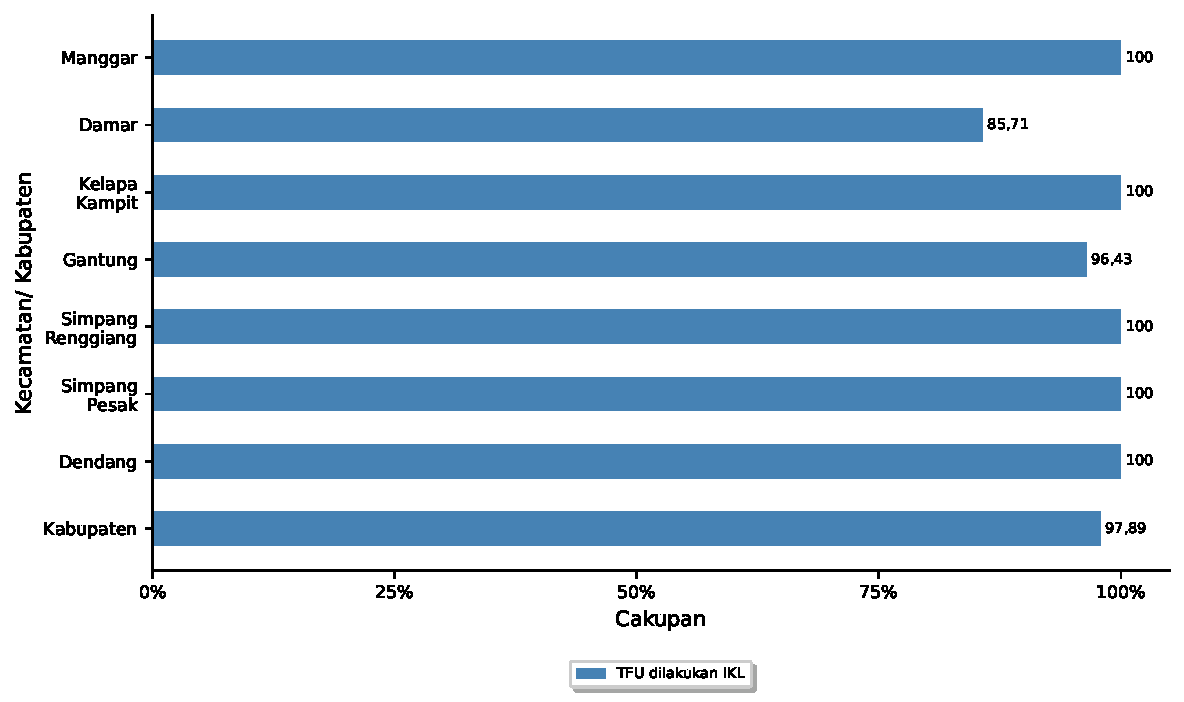
\includegraphics[width=0.85\textwidth]{bab_07/bab_07_04_TFUIKL}
    \caption{Cakupan TFU dilakukan IKL di Kab. Belitung Timur Tahun \tP per Kecamatan}
    \label{fig:Cakupan-TFU-IKL}
\end{figure}

Dari 142 TFU yang ada di Kabupaten Belitung Timur pada tahun \tP,
sebanyak 121 tempat atau 85,21\% di antaranya telah dilakukan IKL (\autoref{fig:Cakupan-TFU-IKL}).

\section{PENGAWASAN TEMPAT PENGELOLAAN PANGAN}
Tempat Pengelolaan Pangan olahan siap saji yang selanjutnya disebut TPP adalah sarana produksi untuk menyiapkan, mengolah, mengemas, menyimpan, menyajikan dan/atau mengangkut pangan olahan siap saji baik yang bersifat komersial maupun non komersial.

TPP yang menjadi sasaran prioritas pengawasan dan pembinaan adalah TPP komersial.

TPP komersial adalah usaha penyediaan pangan siap saji yang memperdagangkan produknya secara rutin, yaitu jasa boga/ketering, restoran, TPP tertentu, depot Air Minum (DAM), rumah makan, gerai pangan jajanan, gerai pangan jajanan keliling, dapur gerai pangan jajanan, dan sentra gerai pangan jajanan/kantin.

TPP dinyatakan sehat bila telah memenuhi persyaratan higiene sanitasi sesuai dengan peraturan yang berlaku dibuktikan dengan dikeluarkannya sertifikat laik higiene sanitasi pangan (HSP).

Pada tahun \tP{}, jasa boga laik HSP adalah sebesar 63,64\%, restoran laik HSP adalah sebesar 100\%, depot air minum laik HSP adalah sebesar 61,19\% rumah makan laik HSP adalah sebesar 10,29\%, gerai jajanan laik HSP adalah sebesar 27,86\%, dan kantin laik HSP adalah sebesar 45,56\%(\autoref{fig:Cakupan-TPP-HSP}). Tidak terdapat TPP Tertentu di Kabupaten Belitung Timur pada tahun \tP .

\begin{figure}[H]
    \centering
    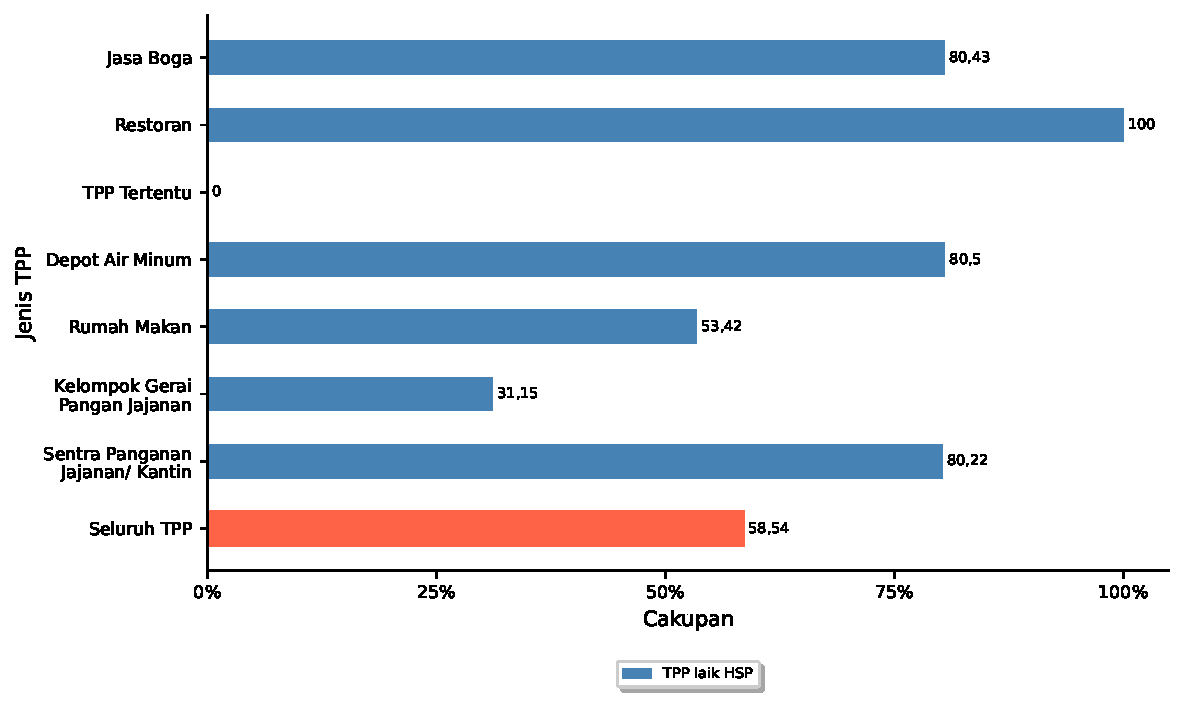
\includegraphics[width=0.85\textwidth]{bab_07/bab_07_05_TPPHSP}
    \caption{Cakupan TPP Laik HSP di Kab. Belitung Timur tahun \tP per Jenis TPP}
    \label{fig:Cakupan-TPP-HSP}
\end{figure}